\documentclass[UTF8,12pt,a4paper,oneside,fontset=none]{ctexrep}

\usepackage{fontspec}
\setmainfont{Times New Roman}
\setCJKmainfont{Songti SC}
\setCJKsansfont{Songti SC}
\setCJKmonofont{Songti SC}

\usepackage[a4paper,margin=2.8cm,includeheadfoot,headheight=24pt,headsep=16pt,footskip=28pt]{geometry}
\usepackage{setspace}
\usepackage{graphicx}
\usepackage{xcolor}
\usepackage{tikz}
\usepackage{booktabs}
\usepackage{array}
\usepackage{amsmath}
\usepackage{csquotes}
\usepackage{float}
\usepackage[section]{placeins}
\usepackage[backend=biber,style=ieee,citestyle=numeric-comp]{biblatex}
\usepackage{fancyhdr}
\usepackage{lastpage}
\usepackage{xurl}
\usepackage[hidelinks]{hyperref}
\usetikzlibrary{arrows.meta,calc,fit,positioning}

\addbibresource{references.bib}
\onehalfspacing
\emergencystretch=2em
\newcolumntype{L}[1]{>{\raggedright\arraybackslash}p{#1}}

\makeatletter
\setlength{\@fptop}{0pt}
\setlength{\@fpsep}{12pt plus 1fil}
\makeatother

\ctexset{
  chapter={name={第,章}},
  section={format=\Large\bfseries},
  subsection={format=\large\bfseries}
}

\fancypagestyle{zhreading}{
  \fancyhf{}
  \fancyhead[L]{Model2Blockly 硕士论文 · 第六章中文阅读版}
  \fancyfoot[C]{第 \thepage\ 页 / 共 \pageref*{LastPage} 页}
  \renewcommand{\headrulewidth}{0.4pt}
  \renewcommand{\footrulewidth}{0pt}
}
\pagestyle{zhreading}

\hypersetup{
  pdftitle={基于现有 Blockly 编辑器的评估——第六章中文阅读版},
  pdfauthor={Xiaoyong Wang},
  pdfsubject={TFM 第六章中文翻译}
}

\begin{document}

% ctex/report may restore the class's plain style at document start; define it
% here so figure-only pages use the same header and footer as the text.
\fancypagestyle{plain}{
  \fancyhf{}
  \fancyhead[L]{Model2Blockly 硕士论文 · 第六章中文阅读版}
  \fancyfoot[C]{第 \thepage\ 页 / 共 \pageref*{LastPage} 页}
  \renewcommand{\headrulewidth}{0.4pt}
  \renewcommand{\footrulewidth}{0pt}
}

\hypersetup{pageanchor=false}
\begin{titlepage}
  \centering
  \vspace*{3cm}
  {\Huge\bfseries 基于现有 Blockly 编辑器的评估\par}
  \vspace{0.8cm}
  {\LARGE 第六章中文阅读版\par}
  \vspace{1.5cm}
  {\large 根据西班牙语论文正文完整翻译；原图、数据与技术标识保持不变\par}
  \vfill
  {\large Xiaoyong Wang\par}
  \vspace{0.5cm}
  {\large 2026 年 7 月\par}
\end{titlepage}

\hypersetup{pageanchor=true}
\pagenumbering{roman}
\tableofcontents
\clearpage
\pagenumbering{arabic}
\setcounter{chapter}{5}
% 第六章中文完整阅读版。
% 译自 chapters/06_casos_uso_evaluacion.tex；原图、技术标识、交叉引用与数据保留。
\chapter{对现有 Blockly 编辑器的评估}
\label{chap:evaluacion}
\label{chap:casos-evaluacion}

上一章介绍了 Model2Blockly 的执行与实现方式。本章转而从另一个视角考察该方案：它能够在多大程度上
用规格描述已有的 Blockly 编辑器，并重新生成这些编辑器。主要证据来自 Blockly 官方仓库中发布的
十种配置。这样，本次评估便将所提出的方案与一组编辑器进行对照，而这些编辑器的结构并非
为了适配 Model2Blockly 的能力而创建。

分析单元是\emph{Blockly 编辑子系统}：块定义、字段、输入、连接、工具箱，以及编辑器自身的
行为。所选应用还包含地图、画布、音频、动画、解释器和模拟器。这些层会使用由块构建的程序，
但它们不属于 Model2Blockly 所生成的编辑器，因此不在评估范围之内。作出这一区分十分必要，
因为不应要求编辑器生成器同时复现集成这些编辑器的特定应用。

本章首先介绍评估问题和语料集，随后定义处理方案、控制变量、规范描述符与评估指标。后续各节
将给出功能方面的结果、规格编写工作量、观察到的局限、Ecore 与 \texttt{.m2b} 输入路线之间的
等价性、效度威胁以及补充技术证据。

\section{评估目标与问题}
\label{sec:objetivo-evaluacion}

评估的目标是确定 Model2Blockly 能否有效创建现有 Blockly 编辑器的编辑子系统，并判断与其
官方源代码相比需要多少规格编写工作量。这里的\emph{有效}并不仅仅意味着 HTML 页面能够打开：
还需要检查编辑器的可观测属性，记录差异，并将匹配项与尚不支持的能力区分开来。

本次评估回答以下四个研究问题；其中 RQ 是英文\emph{research question}（研究问题）的缩写：

\begin{description}
  \item[RQ1 --- 功能复现。] Model2Blockly 能够复现十个编辑器可观测属性中的多大比例？

  \item[RQ2 --- 规格编写工作量。] 与通过 Blockly 的 JSON 或 JavaScript API 实现的官方版本
  相比，开发者必须维护的源代码规模有何变化？

  \item[RQ3 --- 局限。] 官方编辑器的哪些特性无法使用当前的元模型、DSL 和生成器来表达，
  或者只能得到部分表达？

  \item[RQ4 --- 输入路线。] 对于一个简单样例、一个中等样例和一个复杂样例，Ecore 与
  \texttt{.m2b} 输入路线是否会生成相同的规范描述符？
\end{description}

RQ1（功能复现）与 RQ3（局限）评估可观测覆盖范围；RQ2（规格编写工作量）比较可维护、可复现
的产物；RQ4（输入路线）检验两种输入的内部一致性。本研究不测量开发时间，因为这些模型是在
研究本身的开发过程中构建的，这样得到的时间数据并不构成受控的人因实验。本研究也不评估
最终用户的学习效果或可用性。

\section{现有编辑器语料集}
\label{sec:corpus-evaluacion}

本语料集汇集了 Blockly Games 官方目录中列出的八个应用程序---Puzzle、Maze、Bird、Turtle、
Movie、Music、Pond Tutor 和 Pond---以及官方 \texttt{blockly-samples} 仓库中的两个演示：
Graph Demo 与 JS-Interpreter Wait
\cite{blocklyGamesCatalogue,blocklyGamesRepository,blocklySamplesRepository}。
这一选择是有意为之：它涵盖的范围从只有一个块的编辑器，一直到包含工具箱、自定义字段、
变形器（\emph{mutators}）、初始配置和数十种块类型的编辑器。本语料集并不声称是从所有使用
Blockly 构建的编辑器中随机抽取的样本。

有些应用会根据关卡调整工具箱。在这些情况下，本研究固定采用能够展示最完整且最稳定的能力
集合、同时又不改变编辑器模式的配置。Pond Tutor 使用第 9 关，因为奇数关会显示 Blockly，
而该关是这种模式下的最后一关。Puzzle 不使用常规工具箱，因此通过其初始工作区进行评估。
表 \ref{tab:corpus-blockly} 汇总了十个具体的分析单元。

\begin{table}[htbp]
  \centering
  \scriptsize
  \setlength{\tabcolsep}{3.5pt}
  \begin{tabular}{@{}
      L{0.13\textwidth}
      L{0.19\textwidth}
      L{0.36\textwidth}
      L{0.12\textwidth}
      >{\raggedleft\arraybackslash}p{0.08\textwidth}@{}}
    \toprule
    案例 & 编辑器 & 固定配置 & 复杂度 & 块数量 \\
    \midrule
    E01 & Graph Demo & 完整演示。 & 简单 & 2 \\
    E02 & JS-Interpreter Wait & 使用 \texttt{wait\_seconds} 的异步演示。
      & 简单 & 1 \\
    E03 & Maze & 第 10 关，最大且稳定的工具箱。 & 中等 & 5 \\
    E04 & Bird & 第 10 关，最大工具箱。 & 中等 & 8 \\
    E05 & Movie & 第 10 关，自由编辑模式。 & 中等 & 5 \\
    E06 & Music & 第 10 关，完整工具箱。 & 复杂 & 6 \\
    E07 & Turtle & 第 10 关，自由编辑模式。 & 复杂 & 12 \\
    E08 & Puzzle & 初始工作区，无常规工具箱。
      & 复杂 & 3 \\
    E09 & Pond Tutor & 第 9 关，教程中最后一个 Blockly 配置。
      & 复杂 & 11 \\
    E10 & Pond & 完整的 Pond Duck 编辑器。 & 复杂 & 24 \\
    \bottomrule
  \end{tabular}
  \caption{评估所使用的官方配置语料集}
  \label{tab:corpus-blockly}
\end{table}

为保证可复现性，每次运行都不会获取最新版本的源代码。Blockly Games 固定在标识为
\texttt{5d2ff6f39207} 的修订版本，\texttt{blockly-samples} 则固定在
\texttt{62ce12097707}；完整哈希值保存在实验清单中。每个提取出的代码片段都会记录仓库、路径、
行号范围和 SHA-256 哈希值。这样一来，即使项目的主分支持续演化，也可以验证比较时使用的
参照版本是否完全相同。

\section{分析单元与范围}
\label{sec:alcance-evaluacion-externa}

评估针对每个应用区分以下三个层次：

\begin{enumerate}
  \item \textbf{Blockly 编辑器}：块类型、文本、字段、输入、连接、颜色、帮助信息、工具箱、
  初始配置，以及会改变编辑过程的动态行为；
  \item \textbf{代码生成}：与块关联的生成器是否存在及其声明式结构；这部分单独报告；
  \item \textbf{领域应用}：解释、模拟、地图、画布、音频、动画、评分，以及编辑器之外的导航。
\end{enumerate}

第一层构成 RQ1（功能复现）的主要评估指标。第二层单独处理，以免因为块的形状正确便认定其
代码也能完整执行。第三层则排除在外。例如，对于 Maze，本研究比较第 10 关的五个块和工具箱，
但不比较地图或 Pegman 的动画；对于 Turtle，比较的是绘图块，而不是解释这些块指令的画布；
对于 Music，则不复现音频引擎。

还必须将 Blockly 的渲染器（\emph{renderer}）与领域可视化区分开来。Geras 或 Zelos 是内部
渲染器，用来决定 Blockly 如何绘制块的几何形状。Maze 的地图或 Turtle 的画布则属于宿主应用
的层次。在实验中，Geras 被固定为控制变量，而领域可视化则排除在评估之外。

编辑器范围内包括标识符、可见顺序、字段的类与值、类型检查、连接、布局、颜色、工具提示、
帮助链接、类别、工具箱条目、阴影块、预配置值、变形器、验证器以及动态形状变化。当某项纳入
范围的能力无法由 Model2Blockly 表达时，不会将其从分母中移除；它会被记录为差异，并计入
RQ3（方案的局限）。

\section{实验设计}
\label{sec:diseno-experimental-blockly}

\subsection{处理方案与控制变量}

每个案例都构建以下两种处理方案：

\begin{itemize}
  \item \textbf{BASELINE（基线）}：官方编辑子系统定义中未经修改的源代码片段；
  \item \textbf{M2B}：为该案例维护的 \texttt{.m2b} 模型，以及通过 Model2Blockly 实际工具链
  生成的编辑器。
\end{itemize}

两种处理方案都加载到同一个测试容器中；该容器使用 Blockly 13.1.1、Geras 渲染器、Classic
主题、英语区域设置、1280~$\times$~800 像素的窗口，以及 1024~$\times$~640 像素的工作区。
依赖项安装在本地，不会从 CDN 获取版本不固定的依赖。当旧版源代码需要进行调整才能兼容
Blockly 13.1.1 时，适配代码会保存在单独文件中并加以记录，而且不计入官方代码量。

Graph、Maze 和 Turtle 还包含一种 \textbf{ECORE} 处理方案，三者分别代表简单、中等和复杂案例。
其作用是回答 RQ4（输入路线）：ECORE 与 M2B 描述同一个编辑器，并对两者的结果
进行比较；ECORE 不会取代官方基线（BASELINE）。

图 \ref{fig:flujo-evaluacion-externa} 对该流程进行了概括。主要比较是在官方规范描述符与由
\texttt{.m2b} 生成的规范描述符之间进行的。Ecore 检查是针对三个案例的额外配对比较，不会
改变十个编辑器的评估指标。

\begin{figure}[htbp]
  \centering
  \resizebox{0.98\textwidth}{!}{%
  \begin{tikzpicture}[
      node distance=0.55cm and 0.85cm,
      source/.style={draw=black!55, rounded corners=2pt, fill=green!8,
        minimum width=3.1cm, minimum height=0.75cm, align=center, font=\small},
      process/.style={draw=black!55, rounded corners=2pt, fill=blue!7,
        minimum width=3.2cm, minimum height=0.75cm, align=center, font=\small},
      result/.style={draw=black!55, rounded corners=2pt, fill=orange!10,
        minimum width=3.25cm, minimum height=0.75cm, align=center, font=\small},
      arrow/.style={-{Latex[length=2.4mm]}, thick, draw=black!70}
    ]
    \node[source] (official) {官方源代码\\基线（BASELINE）};
    \node[source, below=of official] (m2b) {案例模型\\\texttt{.m2b}};
    \node[source, below=of m2b] (ecore) {等价模型\\Ecore (E01, E03, E07)};

    \node[process, right=of official] (officialHarness)
      {受控 Blockly\\容器};
    \node[process, right=of m2b] (m2bGeneration)
      {Model2Blockly 生成\\+ 受控容器};
    \node[process, right=of ecore] (ecoreGeneration)
      {Model2Blockly 生成\\+ 受控容器};

    \node[result, right=of officialHarness] (officialDescriptor)
      {官方规范\\描述符};
    \node[result, right=of m2bGeneration] (m2bDescriptor)
      {M2B 规范\\描述符};
    \node[result, right=of ecoreGeneration] (ecoreDescriptor)
      {Ecore 规范\\描述符};

    \node[result, right=1.05cm of m2bDescriptor] (comparison)
      {结果\\比较};

    \draw[arrow] (official) -- (officialHarness);
    \draw[arrow] (m2b) -- (m2bGeneration);
    \draw[arrow] (ecore) -- (ecoreGeneration);
    \draw[arrow] (officialHarness) -- (officialDescriptor);
    \draw[arrow] (m2bGeneration) -- (m2bDescriptor);
    \draw[arrow] (ecoreGeneration) -- (ecoreDescriptor);
    \draw[arrow] (officialDescriptor.east) -- ++(0.42,0) |- (comparison.north);
    \draw[arrow] (m2bDescriptor) -- (comparison);
    \draw[arrow] (ecoreDescriptor.east) -- ++(0.42,0) |- (comparison.south);
  \end{tikzpicture}%
  }
  \caption{外部评估中的处理方案与比较}
  \label{fig:flujo-evaluacion-externa}
\end{figure}

\subsection{规范描述符与比较规则}

容器将每种处理方案转换为一个独立于其源语法的 JSON 描述符。该描述符
记录运行控制参数、块、工具箱、初始工作区、生成器和加载错误。每个块会进一步
分解为原子属性：输入顺序、字段、类型检查、连接、布局、颜色、帮助提示文本、
帮助链接和动态行为。JSON 属性的排列顺序无关紧要，但字段、输入、类别及
工具箱元素的可见顺序会被保留。

每个观测到的属性都会被赋予以下状态之一：

\begin{itemize}
  \item \texttt{match}：值和可观测行为等价；
  \item \texttt{partial}：对同一能力的近似实现，但存在一项有明确记录的具体差异；
  \item \texttt{mismatch}：该能力存在，但生成的值不一致；
  \item \texttt{unsupported}：当前生成链中不存在相应表示；
  \item \texttt{error}：生成的块或编辑器无法加载；
  \item \texttt{excluded}：观测到的差异属于已排除的执行层，不计入分母。
\end{itemize}

每项初步判定为有差异的属性都必须对应唯一一条评估规则，由该规则说明相关能力、
涉及的局限及理由。如果某项差异没有对应规则、同一属性适用两条规则，或某条
规则已不再与结果相符，验证都会失败。这一条件可以防止为了提高最终数值而悄然
重新归类某项差异。

RQ1（功能复现）的主要指标为：

\begin{equation}
  \text{编辑器一致率} =
  \frac{\text{状态为 \texttt{match} 的属性}}
       {\text{可适用属性}} \times 100.
  \label{eq:paridad-editor}
\end{equation}

分母包括 \texttt{match}、\texttt{partial}、\texttt{mismatch}、
\texttt{unsupported} 和 \texttt{error}。\texttt{excluded} 差异会单独
报告。某案例在无错误且达到 100\,\% 时归类为\emph{完整}；能够加载但仍
存在差异时归类为\emph{部分复现}；编辑器或其主要块无法加载时则归类为
\emph{不可复现}。生成器采用相同的状态，但其一致率不计入编辑器的主要得分，
而是另行报告。

\subsection{规格编写工作量指标}

RQ2（规格编写工作量）比较的是需要维护的源文件，而非生成的输出。在 BASELINE
中，只统计该配置所需的定义、编辑器扩展、工具箱构造和生成器。许可证、导入、
容器 HTML、翻译、领域引擎和程序库均排除在外。在 M2B 中统计
\texttt{source.m2b} 文件；生成的 JavaScript 和 HTML 不纳入度量。

对于两种处理方案，都会记录 UTF-8 字节数、总行数、非空行数以及不含注释的
非空行数。主要比较采用最后一种单位：

\begin{equation}
  \text{LOC 缩减率} =
  \left(1 - \frac{\text{LOC}_{\mathrm{m2b}}}
                    {\text{LOC}_{\text{官方}}}\right) \times 100.
  \label{eq:reduccion-loc}
\end{equation}

本文给出各案例的数值、均值、中位数和加权总计。Pond Tutor 和 Pond 复用了
相同官方文件中的若干行。因此，除了将十种配置作为独立产物相加之外，还会计算
一个保守总计，并逐行去重：仅当仓库、修订版本、路径和行号全部相同时，才将该行
官方代码视为重复。十个 \texttt{.m2b} 模型仍保留在该计算中，因为它们是作为独立规格
分别维护的。

Ecore 被有意排除在这一指标之外。将 XML/XMI 的 LOC 与 DSL 的 LOC 比较，
会混合不同的编辑单位。在 RQ4（输入路线）中，Ecore 与 \texttt{.m2b} 的
描述符必须在运行控制参数、块、工具箱、初始工作区、生成器、错误和可加载性方面严格
相同；结果只有等价或不等价两种，并同时给出可能存在的差异。

\section{评估流程与可复现性}
\label{sec:procedimiento-evaluacion-blockly}

每个案例均遵循同一流程：

\begin{enumerate}
  \item 锁定仓库、修订版本和具体配置；
  \item 确定纳入范围的官方代码片段；
  \item 在不作修改的情况下将其提取出来，并核验行号区间和哈希；
  \item 编写该编辑器的 \texttt{.m2b} 模型；
  \item 执行实际生成链；
  \item 在相同的浏览器受控环境下加载 BASELINE 和 M2B；
  \item 实例化各个块并取得规范描述符；
  \item 比较描述符属性，并要求每项差异都有唯一的理由；
  \item 使用同一个度量程序收集 LOC 和字节数；
  \item 保存 JSON 结果和截图，作为可复现证据。
\end{enumerate}

截图可用于检查各处理方案能否正常加载并呈现预期的块，但不作为像素级等价的
证据。判定依据是结构属性和浏览器观测到的错误。对于 E01、E03 和 E07，随后
还会增加 Ecore 生成，并要求其描述符与 M2B 描述符完全相同。

语料集、控制变量和修订版本均在清单
\path{evaluation/official-blockly/}\allowbreak\path{manifest.json} 中声明。
每个案例目录包含官方代码提取结果、\path{source.m2b}、生成输出、评估规则、
描述符、指标和截图。命令 \texttt{npm run\allowbreak{} verify:\allowbreak{}evaluation-\allowbreak{}completed}
会运行容器和全部十个案例；\texttt{npm run\allowbreak{} aggregate:\allowbreak{}evaluation} 会重新生成
全局汇总。保留各案例的单独结果，既可以防止均值掩盖个别案例，也可以将每项
局限追溯到具体属性。

前两个案例 Graph 和 Maze 被用作试点，以便在完成整个语料集之前确定描述符模式、
字段匹配方式和比较状态。标准确定后，便以相同粒度应用于其余八个案例。下一节将
介绍使用这一协议得到的结果。

\section{功能复现结果}
\label{sec:resultados-reproduccion}

表~\ref{tab:resultados-casos-blockly} 汇总了各案例的结果。“编辑器”列衡量
块和工具箱的结构属性；“生成器”列衡量纳入范围的生成属性。两列都以“匹配数/
可适用属性数”的形式显示。范围之外的差异不计入分母。最后三列比较官方配置的
LOC 与 \texttt{.m2b} 模型的 LOC。

\begin{table}[htbp]
  \centering
  \caption{各案例结果：功能一致率与规格编写工作量}
  \label{tab:resultados-casos-blockly}
  \resizebox{\textwidth}{!}{%
  \begin{tabular}{llrrrrrrrr}
    \toprule
    案例 & 编辑器 & 块数 & 编辑器 $m/a$ & 编辑器（\%） & 生成器 $m/a$ & 生成器（\%） & 官方 LOC & M2B LOC & 缩减率（\%） \\
    \midrule
    E01 & Graph       &  2 &  77/91  & 84,62 &  7/8   & 87,50 & 329 &  28 & 91,49 \\
    E02 & Wait        &  1 &  73/89  & 82,02 &  4/4   & 100,00 & 282 &  16 & 94,33 \\
    E03 & Maze        &  5 & 111/137 & 81,02 & 15/15  & 100,00 & 178 &  73 & 58,99 \\
    E04 & Bird        &  8 & 203/218 & 93,12 & 27/31  & 87,10 & 246 &  93 & 62,20 \\
    E05 & Movie       &  5 & 236/283 & 83,39 & 16/20  & 80,00 & 449 &  75 & 83,30 \\
    E06 & Music       &  6 & 186/232 & 80,17 & 19/21  & 90,48 & 545 &  94 & 82,75 \\
    E07 & Turtle      & 12 & 349/427 & 81,73 & 30/40  & 75,00 & 669 & 190 & 71,60 \\
    E08 & Puzzle      &  3 &  59/75  & 78,67 &  6/12  & 50,00 & 221 &  46 & 79,19 \\
    E09 & Pond Tutor  & 11 & 340/397 & 85,64 & 35/44  & 79,55 & 415 & 154 & 62,89 \\
    E10 & Pond        & 24 & 681/813 & 83,76 & 68/96  & 70,83 & 740 & 352 & 52,43 \\
    \midrule
    总计 & & 77 & 2315/2762 & 83,82 & 227/291 & 78,01 & 4074 & 1121 & 72,48 \\
    \bottomrule
  \end{tabular}%
  }
\end{table}

编辑器共有 2762 项可适用属性，其中 2315 项匹配，对应的加权一致率为
83,82\,\%。各案例未加权均值为 83,41\,\%，中位数为 82,71\,\%。其范围
从 Puzzle 的 78,67\,\% 到 Bird 的 93,12\,\%。20 个 BASELINE/M2B
处理实例均无错误加载，模型声明的所有块都能成功实例化。不过，十个案例中没有
任何一个达到 100\,\%：它们都被归类为\emph{部分复现}，而非完全等价。

表~\ref{tab:estados-agregados} 所示的状态汇总分布揭示了单一分数会掩盖的
信息。具体而言，编辑器的 366 项属性和生成器的 50 项属性目前仍无法通过通用
规格表达。编辑器的八项 \texttt{mismatch} 对应于对保留块的重新定义；
生成器的六项则集中在 Puzzle 的自动序列化上。

\begin{table}[htbp]
  \centering
  \caption{比较状态的汇总分布}
  \label{tab:estados-agregados}
  \begin{tabular}{lrr}
    \toprule
    状态 & 编辑器 & 生成器 \\
    \midrule
    \texttt{match}       & 2315 & 227 \\
    \texttt{partial}     &   73 &   8 \\
    \texttt{mismatch}    &    8 &   6 \\
    \texttt{unsupported} &  366 &  50 \\
    \texttt{error}       &    0 &   0 \\
    \texttt{excluded}    &    0 &  17 \\
    \bottomrule
  \end{tabular}
\end{table}

图~\ref{fig:evidencia-visual-corpus} 展示了两组有代表性的对比：复杂度中等的
Maze，以及语料集中规模最大的 Pond。截图证实，两种处理方案都能加载可比较的
工具箱和工作区。不过，截图无法取代结构比较：两幅视觉上相近的截图仍可能掩盖
连接、字段内部值或生成器方面的差异。

\begin{figure}[p]
  \centering
  \begin{minipage}{0.48\textwidth}
    \centering
    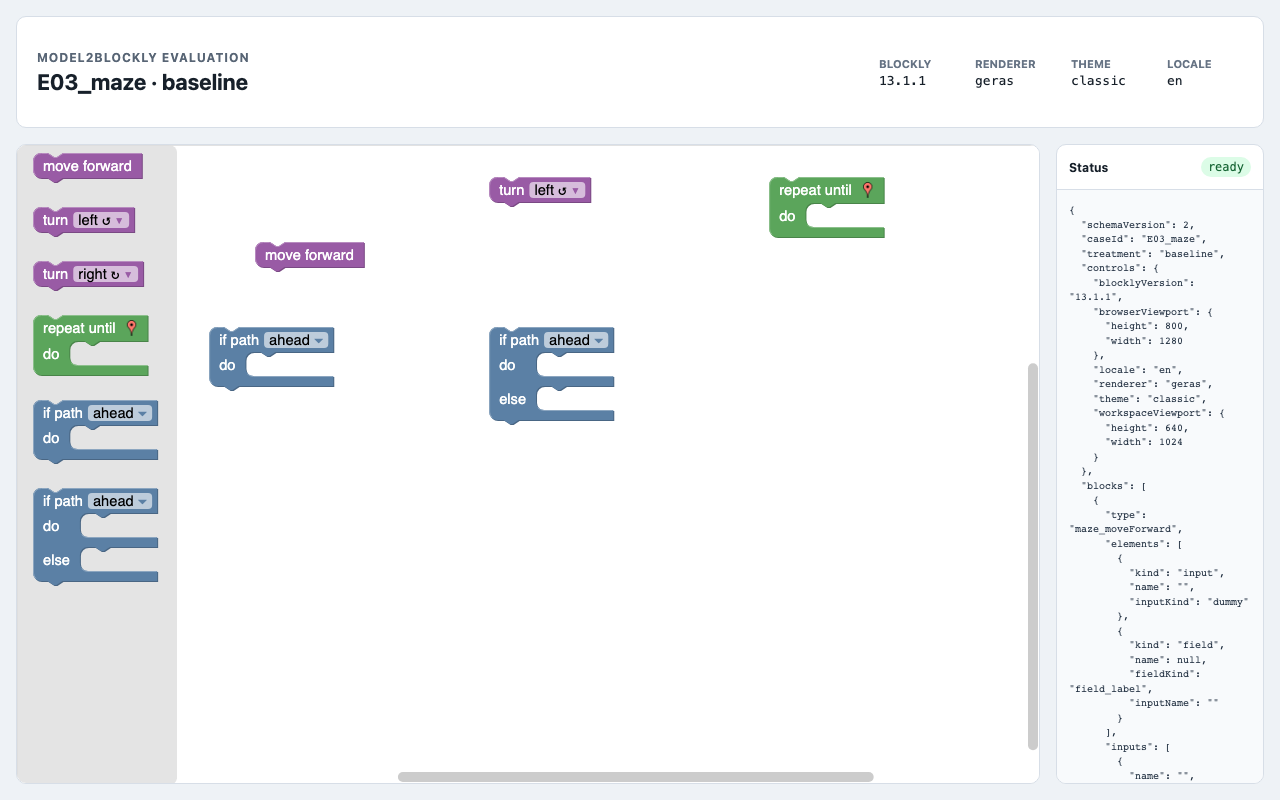
\includegraphics[width=\linewidth]{../../evaluation/official-blockly/cases/E03_maze/results/screenshots/baseline.png}
    \\[2pt]\small (a) 官方 Maze
  \end{minipage}\hfill
  \begin{minipage}{0.48\textwidth}
    \centering
    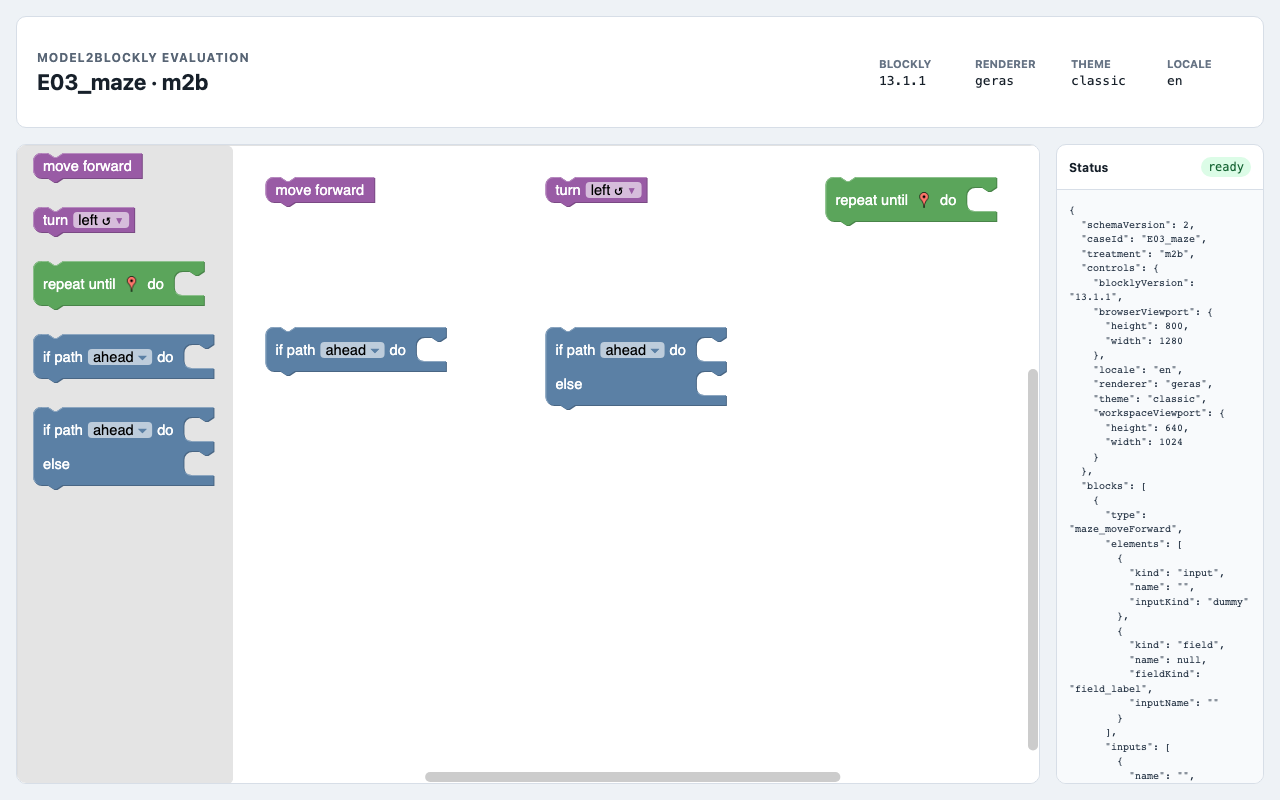
\includegraphics[width=\linewidth]{../../evaluation/official-blockly/cases/E03_maze/results/screenshots/m2b.png}
    \\[2pt]\small (b) 由 M2B 生成的 Maze
  \end{minipage}

  \vspace{0.8em}

  \begin{minipage}{0.48\textwidth}
    \centering
    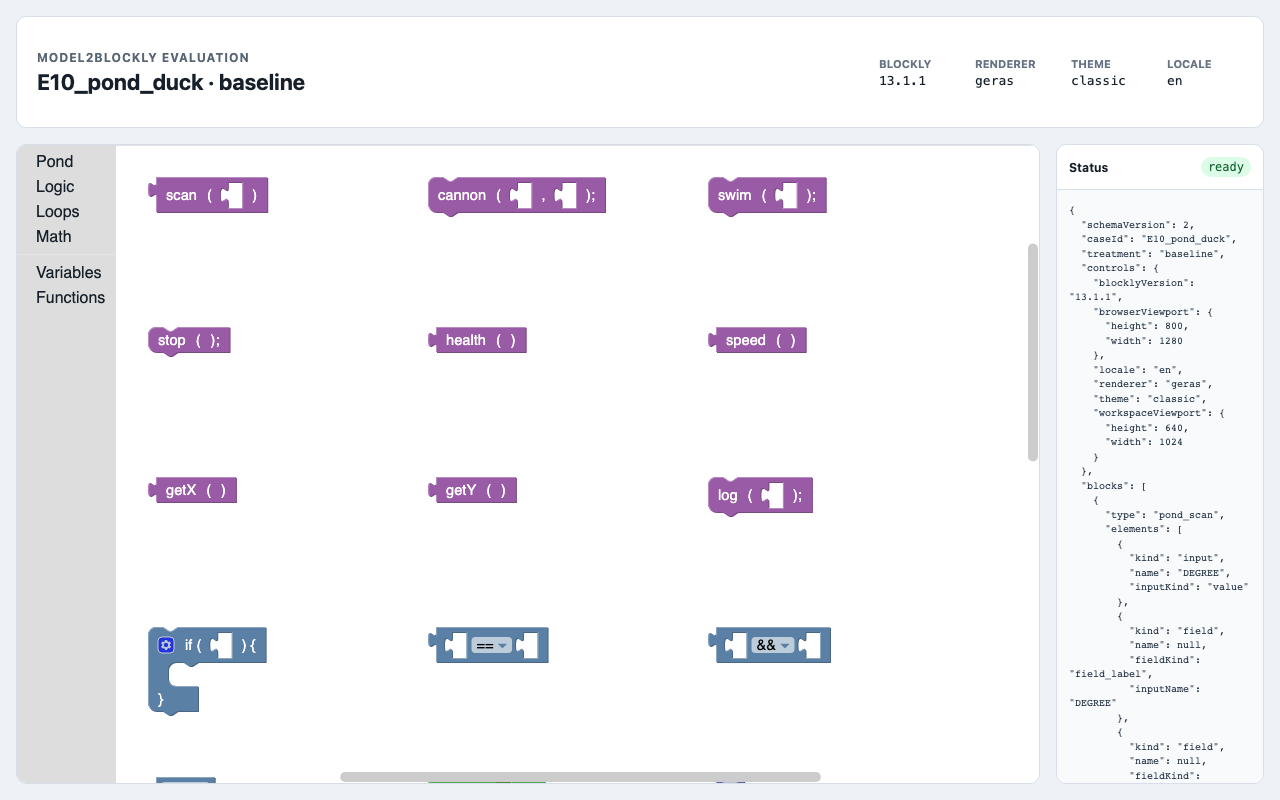
\includegraphics[width=\linewidth]{../../evaluation/official-blockly/cases/E10_pond_duck/results/screenshots/baseline.png}
    \\[2pt]\small (c) 官方 Pond
  \end{minipage}\hfill
  \begin{minipage}{0.48\textwidth}
    \centering
    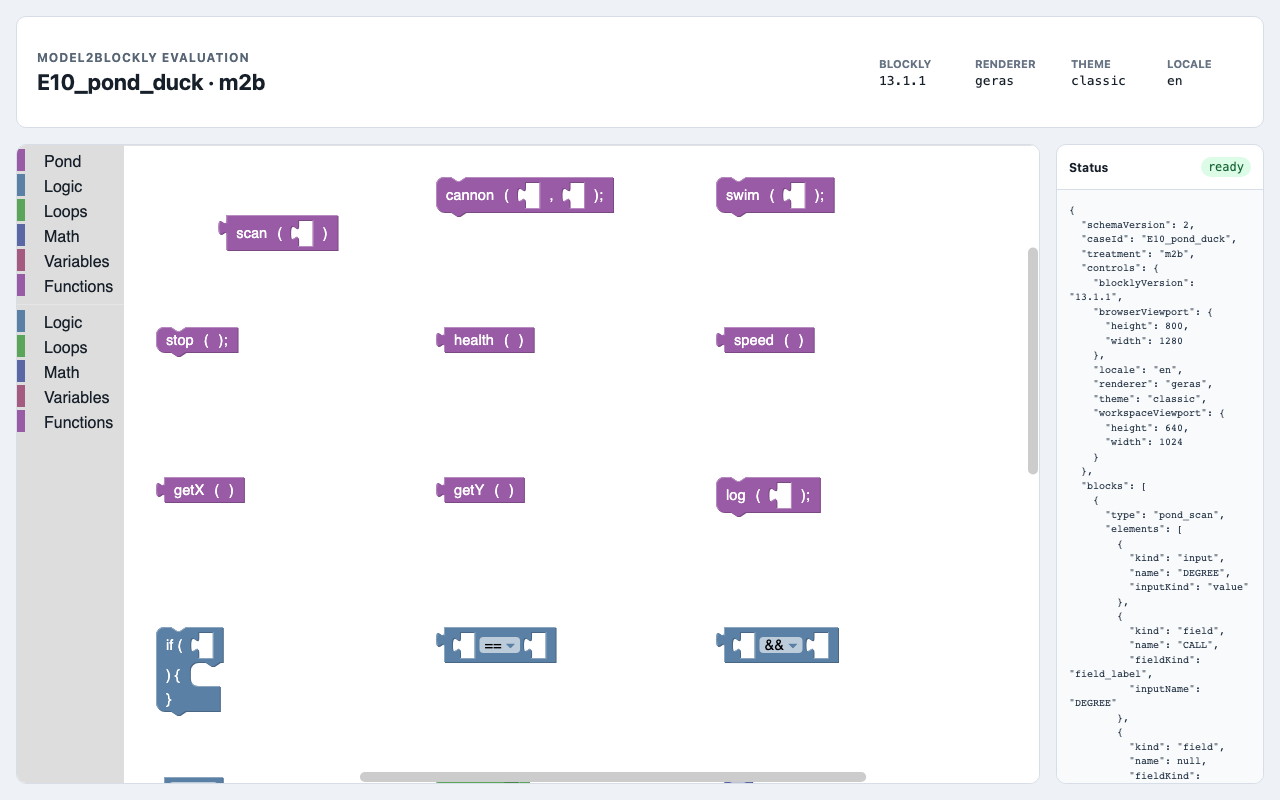
\includegraphics[width=\linewidth]{../../evaluation/official-blockly/cases/E10_pond_duck/results/screenshots/m2b.png}
    \\[2pt]\small (d) 由 M2B 生成的 Pond
  \end{minipage}
  \caption{语料集中两个案例的辅助视觉证据}
  \label{fig:evidencia-visual-corpus}
\end{figure}

\subsection{生成器结果}

生成器的加权一致率为 227/291，即 78,01\,\%。各案例均值为 82,05\,\%，
中位数为 83,55\,\%。有十七项属性标记为 \texttt{excluded}：它们属于
Blockly Games 的执行跟踪和循环中断机制，这些机制会对面向教育应用的程序
进行插桩，但既不定义编辑器，也不定义每种块的基础转换。

Wait 和 Maze 的结果在纳入范围内达到 100\,\%，而 Puzzle 为 50\,\%。
后者得分较低的主要原因是，官方案例会自动序列化整个拼图的状态，而
Model2Blockly 生成的是与块类型关联的函数。此外，Pond 案例中还包含过程、
变量和变形器，它们要求生成期间存在共享状态。因此，这一层得分较低并不意味着
编辑器无法加载，而是说明当前契约并不总能重构官方的生成语义。

\section{规格编写工作量结果}
\label{sec:resultados-esfuerzo}

十个官方配置合计包含 4074 行非空且不含注释的代码（LOC），而
\texttt{.m2b} 模型为 1121 LOC。应用公式~\ref{eq:reduccion-loc} 后，
加权 LOC 缩减率为 72,48\,\%。各案例缩减率的平均值为 73,92\,\%，中位数为
75,40\,\%。按 UTF-8 字节数计算，缩减幅度相近：从 137358 字节降至
40563 字节，即缩减 70,47\,\%。

上述总数将每个编辑器视为可独立维护的产物。为避免 Pond Tutor 与 Pond
之间官方实现中的代码复用使 M2B 获得人为优势，研究剔除共享的官方代码行后重新进行了
计算。此时，保守计算的官方代码总量变为 3737 LOC，缩减率仍达到
70,00\,\%（按字节数计算为 67,67\,\%）。因此，这一趋势并不依赖于对
337 行共享代码进行两次计数。

这一结果需要结合功能一致率来理解。Model2Blockly 大幅缩减了需维护的源代码
规模，但这些模型并不能精确替代所有官方配置。该语料集同时表明，描述工作量
有所减少，并揭示了一组仍然缺失的具体能力；但它并不能证明，只需减少
72,48\,\% 的代码便可实现每个编辑器 100\,\% 的功能。

\section{语料集中观察到的局限}
\label{sec:limites-corpus}

表~\ref{tab:limites-editor} 汇总了编辑器中最常见的差异。这里的计数表示受影响的
原子属性数量，而不是相互独立的特性数量：同一项能力缺失可能会影响一个案例中的
多个块和字段。

\begin{table}[htbp]
  \centering
  \caption{造成主要差异的编辑器能力}
  \label{tab:limites-editor}
  \resizebox{\textwidth}{!}{%
  \begin{tabular}{llrr}
    \toprule
    能力 & 主要状态 & 属性 & 案例 \\
    \midrule
    特定连接策略 & \texttt{unsupported} & 101 & 9 \\
    类别高级组合 & \texttt{unsupported} & 66 & 5 \\
    显式虚拟输入 & \texttt{unsupported} & 52 & 4 \\
    只读调用标签 & \texttt{partial} & 30 & 2 \\
    有意省略类别颜色 & \texttt{unsupported} & 30 & 5 \\
    工具箱整体组合 & \texttt{unsupported} & 19 & 2 \\
    工具箱中的预配置块 & \texttt{unsupported} & 19 & 7 \\
    输入对齐 & \texttt{unsupported} & 14 & 3 \\
    阴影块配置 & \texttt{partial} & 11 & 2 \\
    命名虚拟输入 & \texttt{unsupported} & 11 & 3 \\
    保留块的重新定义 & \texttt{mismatch} & 8 & 3 \\
    \bottomrule
  \end{tabular}%
  }
\end{table}

影响范围最广的局限是连接策略。通用元模型能够表示一个块是否具有输出连接、
前序连接和后继连接，但无法表示官方编辑器通过 JavaScript 添加的所有动态检查与
例外规则。以编程方式构建的工具箱、带初始状态的阴影块、输入的视觉对齐方式，
以及仅用于控制布局的虚拟输入，也都难以处理。这些特性不会阻止编辑器加载，
但会妨碍完整的结构复现。

在生成器方面，最常出现的差异包括：空输入的默认值（六个案例中的 27 个属性）、
枚举映射（三个案例中的 10 个属性）、模型自动序列化（Puzzle 中的六个属性）、
受变形器状态影响的生成（Pond Tutor 和 Pond 中的六个属性），以及过程和变量数据库。
这些观察结果指出了可落实的改进方向：扩展输入与工具箱的元模型，引入声明式连接
策略，并提供有状态的生成服务。

\section{输入路线的等价性}
\label{sec:resultados-rutas-entrada}

RQ4（输入路线）比较的不是 Ecore 与 DSL 的文本规模，而是两个适配器的结果。
研究选择 Graph、Maze 和 Turtle，以逐步覆盖简单字段、连接、下拉菜单、带类别的
工具箱、初始工作区和生成器。在三个案例中，均严格比较了
表~\ref{tab:equivalencia-rutas} 所列规范描述符的七个部分。

\begin{table}[htbp]
  \centering
  \caption{Ecore 与 \texttt{.m2b} 输入路线之间的严格等价性}
  \label{tab:equivalencia-rutas}
  \begin{tabular}{llll}
    \toprule
    案例 & 复杂度 & 已比较部分 & 结果 \\
    \midrule
    E01 Graph  & 简单 & 7/7 & 等价 \\
    E03 Maze   & 中等 & 7/7 & 等价 \\
    E07 Turtle & 复杂 & 7/7 & 等价 \\
    \bottomrule
  \end{tabular}
\end{table}

结果表明，在 3/3 个案例中，两条输入路线均等价：运行控制参数、块、工具箱、初始工作区、
生成器、错误和可加载性
完全一致。该测试也有助于发现实现缺陷。在 Graph 中，研究发现 Ecore 模型缺少
一个 \texttt{output} 注解；在 Turtle 中，则修正了适配器对下拉菜单标签和值的
解释。修正这些问题后，研究重新生成并再次比较了三个完整的配对。并未通过放宽比较器
来使二者匹配。

这一结果表明，对于已覆盖的构造，生成的编辑器并不依赖于模型是使用 Xtext 还是
Ecore 编写的。但该结果不足以断言任意可能的 Ecore 元模型都具有等价性；要进行
这种推广，还需要增加所评估输入路线的数量和多样性。

\section{补充技术证据}
\label{sec:evidencia-complementaria}

除外部评估外，项目还保留了针对实现的测试。六组最小化且彼此互补的
Ecore--\texttt{.m2b} 配对检查了从两类输入到可执行编辑器的完整流程，并验证了
控件、连接、工具箱和生成器的多种变体。专门设计的 Ecore 案例进一步覆盖了没有文本
等价形式的构造。145 项 JUnit 测试覆盖适配器、验证和转换，而通过更新站点进行
安装则验证了插件的打包。

这些测试与语料集评估关注的问题不同。它们为所构建系统的回归、集成和部署提供了证据，
但不作为相对于现有 Blockly 编辑器有效性的主要证明。同样，应用的渲染层---例如迷宫、
画布或音乐模拟---不在主要比较范围之内：Model2Blockly 生成编辑器及其生成器，而不生成
负责执行所产出程序的领域引擎。

\section{效度威胁}
\label{sec:amenazas-validez}

\paragraph{语料集选择。}
十个案例均来自官方代码仓库，并覆盖不同的规模与机制，但它们构成的是一个目的性
样本。这些百分比描述的是该语料集，而不是所有 Blockly 编辑器的统计总体。

\paragraph{依赖项的演化。}
原始编辑器使用较早版本的 Blockly 开发。为避免后续更新改变比较结果，研究固定了
源代码修订版本和 Blockly 13.1.1 版本，并在同一个兼容性容器中运行两个处理方案。
这一结果衡量的是编辑器配置，而不是每个完整应用的历史兼容性。

\paragraph{粒度与分类。}
将评估对象分解为属性并划分为 \texttt{partial}、\texttt{unsupported} 和
\texttt{excluded} 状态，需要做出建模决策。为减少偏差，研究通过两项试点固定了
分类方案，为每项差异指定了一条具有明确标识的规则，并同时公布计数和规范描述符。即便如此，
采用另一种粒度仍可能改变绝对百分比。

\paragraph{产物的独立性。}
Pond Tutor 与 Pond 共享官方源代码。主要计算将二者视为不同的可维护配置，保守
计算则剔除重复代码行。缩减率仍处于 70,00\,\% 至 72,48\,\% 之间，由此可将
这种依赖关系的影响界定在这一范围内。

\paragraph{视觉与语义等价性。}
截图不能证明视觉效果完全相同。评估比较了结构和生成器，但没有穷举运行所有可能的
程序，也没有比较领域引擎的行为。因此，报告的一致率不应被理解为 Blockly Games
应用之间的完全等价性。

\paragraph{工作量度量。}
LOC 和字节数是可复现的源代码规模指标，并不衡量开发时间或认知难度。评估
证明了所维护规格的简洁性；若要断言时间或人力成本也有同等程度的降低，则需要开展
参与者研究。

\section{评估问题的回答}
\label{sec:respuesta-rq}

\begin{table}[htbp]
  \centering
  \caption{评估问题及回答汇总}
  \label{tab:respuesta-rq}
  \footnotesize
  \begin{tabular}{L{0.24\textwidth}L{0.68\textwidth}}
    \toprule
    评估问题 & 评估结论 \\
    \midrule
    \textbf{RQ1：功能复现} & 十个编辑器均可加载；加权结构一致率为 83,82\,\%，生成器一致率为 78,01\,\%。所有案例均被归类为部分复现。 \\
    \textbf{RQ2：规格编写工作量} & M2B 将 LOC 减少了 72,48\,\%；剔除共享的官方源代码后，保守计算的缩减率为 70,00\,\%。 \\
    \textbf{RQ3：局限} & 主要缺失能力涉及连接策略、工具箱组合、呈现用输入，以及带有状态、变形器或自动序列化机制的生成器。 \\
    \textbf{RQ4：输入路线} & 在选定的三个案例中，Ecore 与 \texttt{.m2b} 路线生成严格等价的规范描述符（3/3）。 \\
    \bottomrule
  \end{tabular}
\end{table}

\section{评估结论}
\label{sec:conclusion-evaluacion}

本次评估的证据范围比单个示例更广。对十个官方编辑器的结果表明，\allowbreak{}Model2Blockly
复现了大部分属性，并将需维护的配置源代码减少约 70\,\%。三个
Ecore--\texttt{.m2b} 配对均等价，这进一步支持了适配器与通用规格相分离的设计。
但并未实现完全等价：所有案例仍然存在差异，尤其是在以编程方式构建的工具箱、
变形器或有状态生成方面。因此，该语料集量化了当前覆盖范围、已经实现的缩减幅度，
以及扩大覆盖范围所需的扩展。



\printbibliography[title={参考文献}]

\end{document}
